\subsection{Diseño de la interfaz de usuario}
\label{sec:diseno-ux}

\subsubsection{Introducción}
\label{sec:diseno-ux-introduccion}

La interfaz de usuario es la parte de un programa que interactúa con el usuario. En el caso de \textit{Ott} 
es la parte que se encarga de mostrar la información al usuario y de permitirle interactuar con el sistema
La interfaz de usuario es una parte fundamental de cualquier sistema, ya que es la parte que el usuario ve 
y con la que interactúa. Por tanto, es importante que la interfaz de usuario sea clara, sencilla e intuitiva, 
para que el usuario pueda utilizar el sistema de forma eficiente y sin problemas.

En este apartado se describe como se enfoca las fases de diseño de la interfaz de usuario de \textit{Ott}.

\subsubsection{Diseño de la interfaz de usuario}
\label{sec:diseno-ux-diseno}

Cuando se comenzó con el diseño de de la aplicación, no se trabajó sobre un diseño final exacto ya que este
dependía de los clientes que fueran uniendose al proyecto y decidiendo su propia interfaz. Lo que se fue diseñando
a medida que avanzaba el proyecto fue una interfaz base que permitiera ir añadiendo nuevas funcionalidades y 
los distintos componentes personalizables que se irían añadiendo a la interfaz. 

\begin{figure}[hp!]
    \centering
    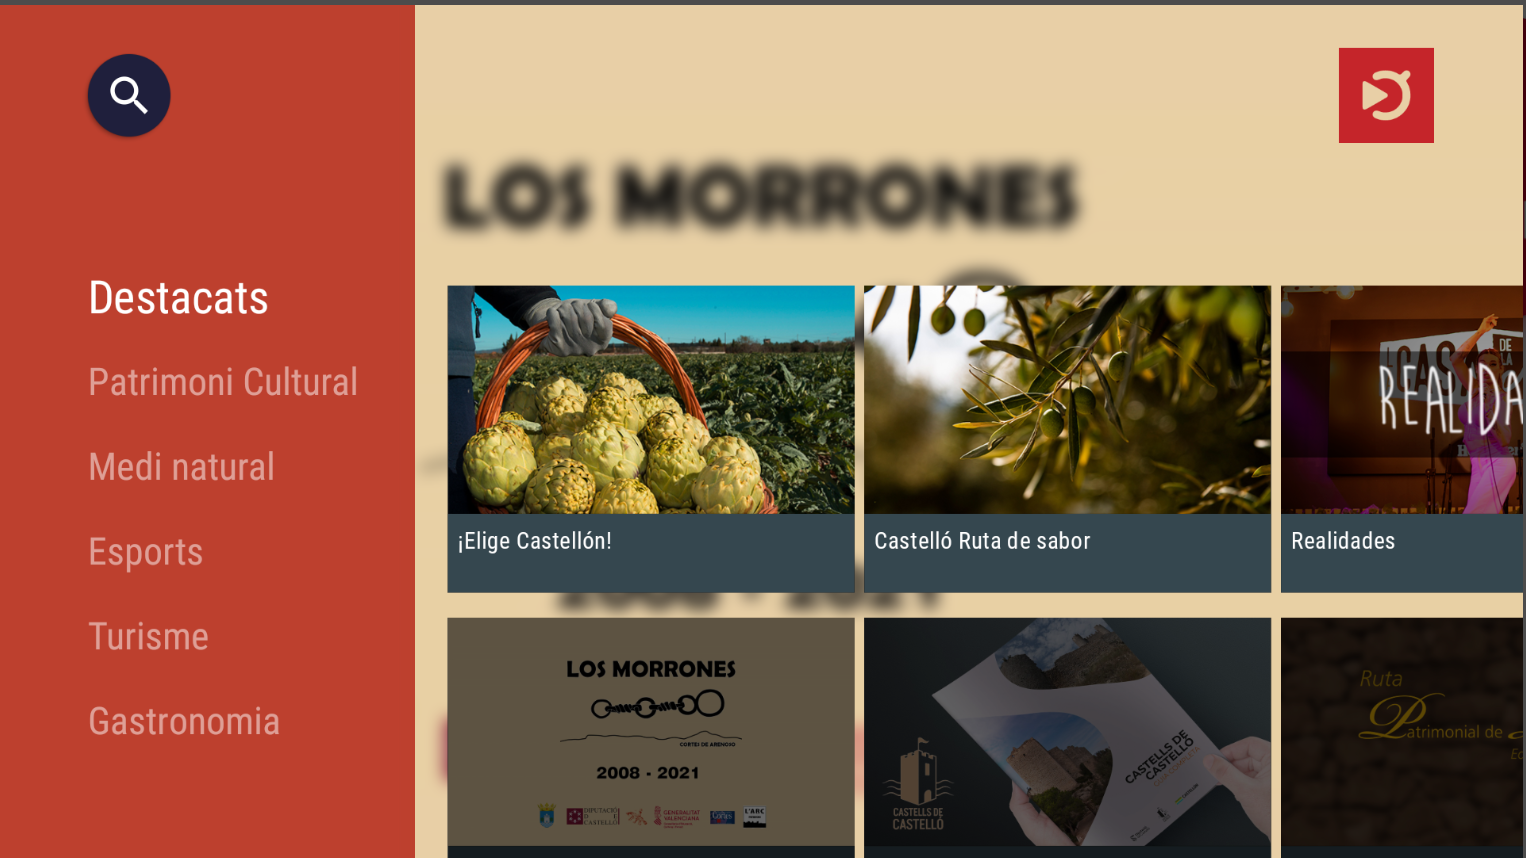
\includegraphics[width=0.8\textwidth]{imaxes/UX_inicios.png}
    \caption{Captura de la interfaz en las primeras fases del proyecto}
    \label{fig:UX_inicios}
\end{figure}
\begin{figure}[hp!]
    \centering
    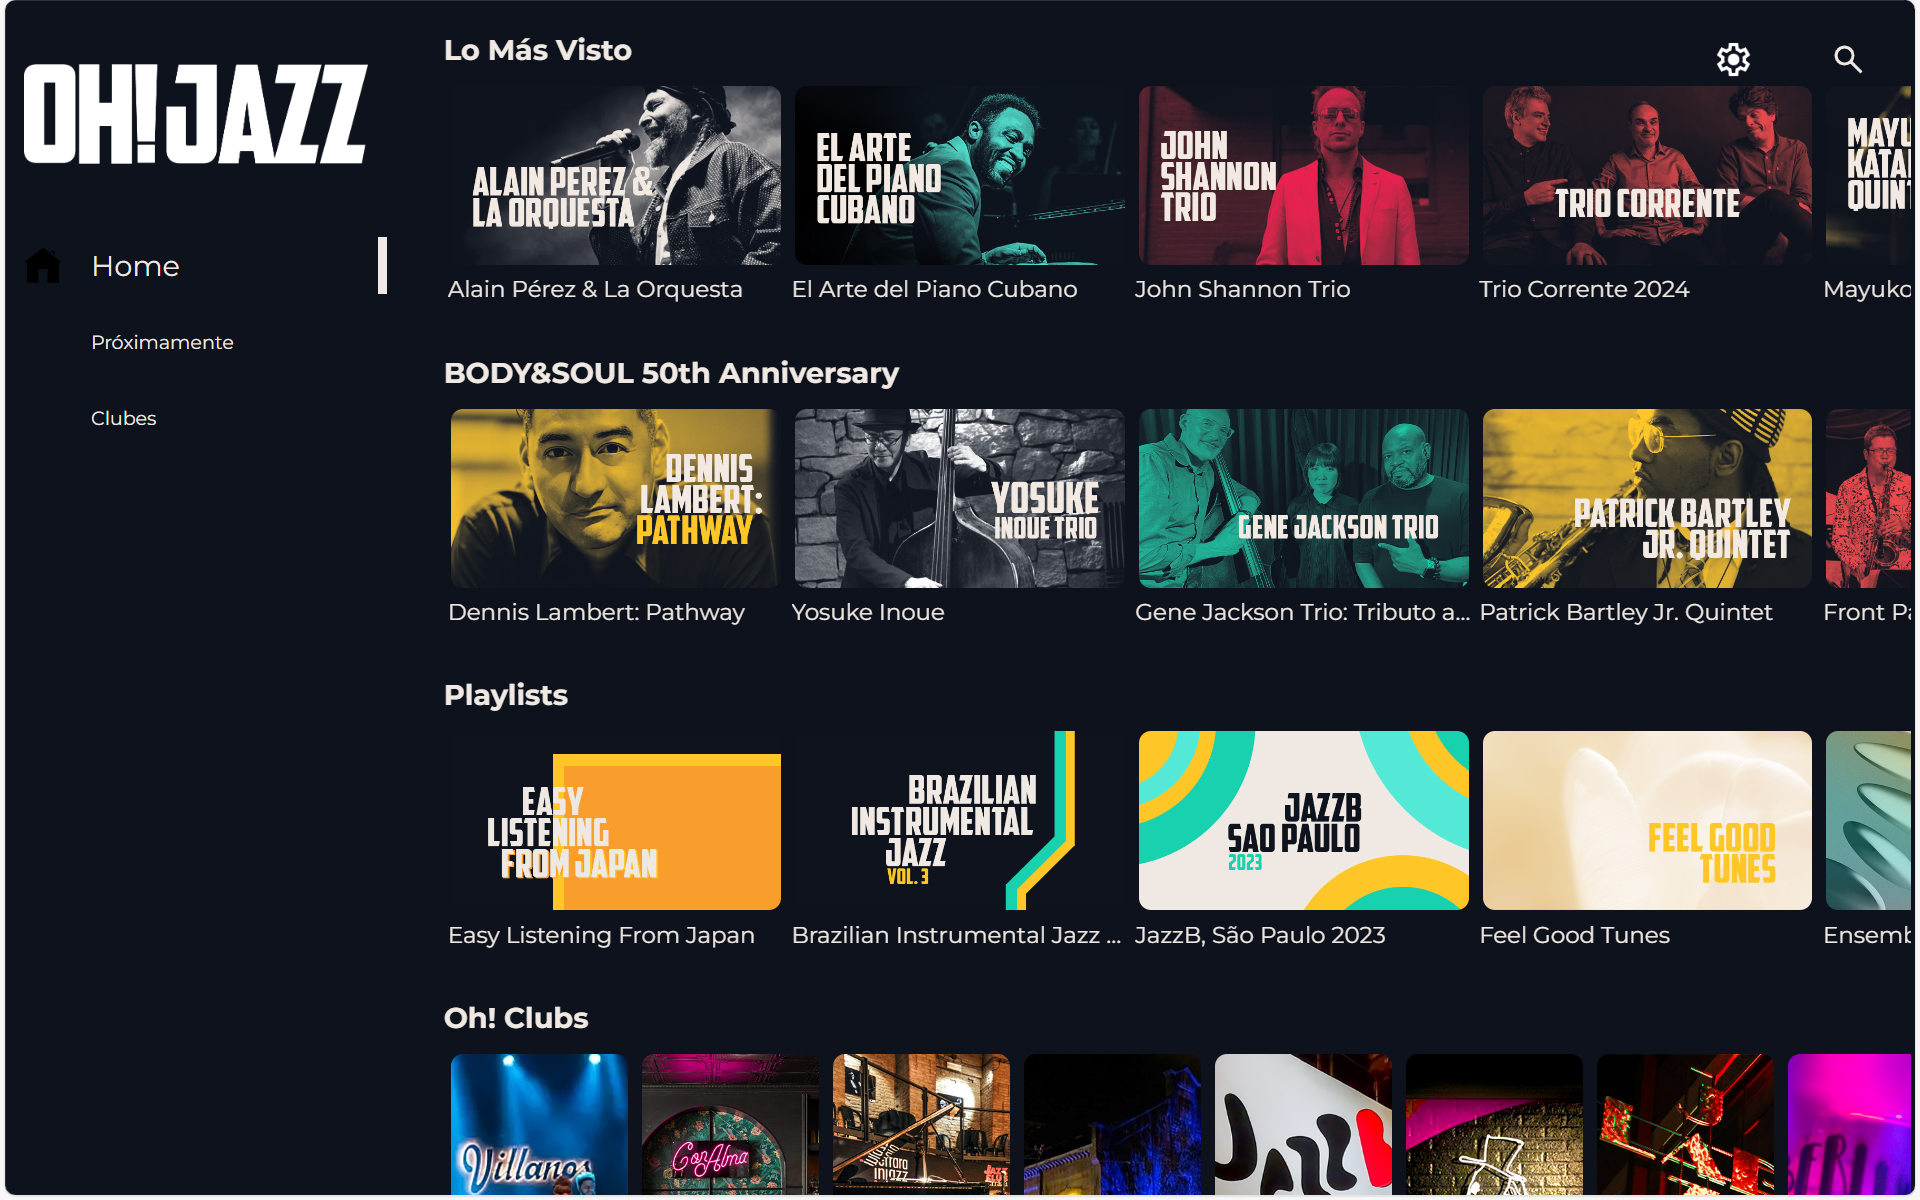
\includegraphics[width=0.8\textwidth]{imaxes/Home_desp_OhJazz.png}
    \caption{Captura de la interfaz más recientes, todavía con pruebas por parte del cliente}
    \label{fig:Home_desp_OhJazz}
\end{figure}
\begin{figure}[hp!]
    \centering
    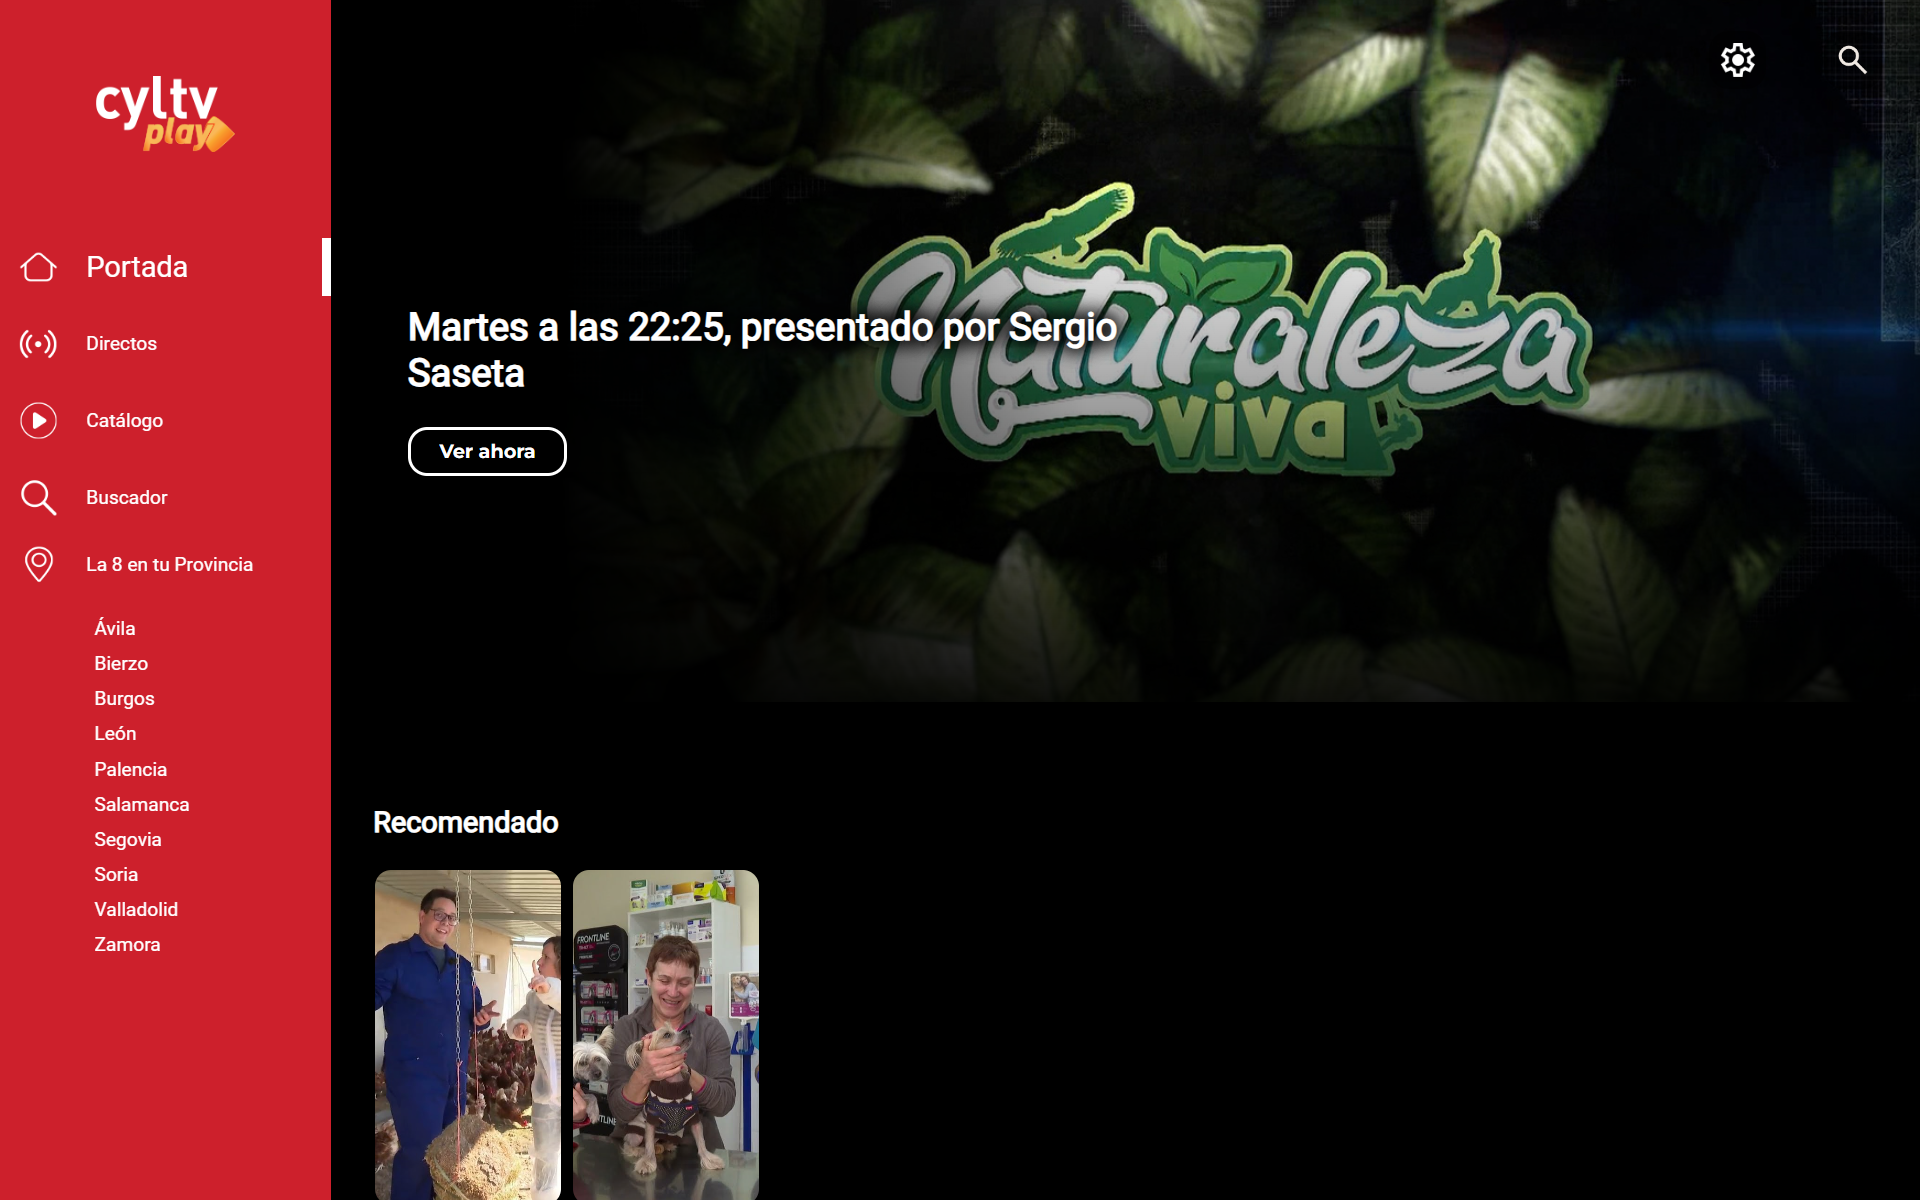
\includegraphics[width=0.8\textwidth]{imaxes/Home_CyLTv.png}
    \caption{Captura de la interfaz casi final}
    \label{fig:Home_CyLTv}
\end{figure}

En estas imagenes se puede apreciar la evolución de la interfaz de usuario de \textit{Ott} desde sus inicios
hasta la versión casi final. En la primera imagen se puede ver la interfaz en sus primeras fases, con un diseño
muy básico y sin apenas funcionalidades. En la segunda imagen se puede ver la interfaz con un diseño más avanzado, 
pero donde el cliente todavía estaba ajustando diferentes parametros (vemos que los iconos de los menús no se ven, 
el menu no contrasta con el fondo, etc). En la tercera imagen se puede ver la interfaz casi final, con un diseño
más pulido y con todas las funcionalidades implementadas.

Más que un diseño como tal de la interfaz, lo que se ha hecho es centrarse en los diseños de los diferentes componentes y sus
variantes. 
La estructura general, los tamaños y posiciones de los componentes principales es la misma (de momento) para todos los clientes, pudiendo
modificar los colores y los textos. Estos componentes son los siguientes:

\begin{itemize}
    \item Menú lateral: es el menú que se encuentra a la izquierda de la pantalla y que permite al usuario navegar por las diferentes secciones de la aplicación.
    \item Menú superior: es el menú que se encuentra en la parte superior de la pantalla y que permite al usuario acceder a las opciones de configuración de la aplicación. 
    Para este componente se pueden llegar a modificar los iconos y los colores de fondo por parte del cliente, pero la posición (depende del número de 
    opciones de este menú) y la funcionalidad es la misma para todos los clientes.
    \item Barra de búsqueda: es la barra que se encuentra en la pantalla de búsqueda y que permite al usuario buscar elementos en la aplicación.
    Esta barra utiliza los colores base del cliente para el difuminado y foco, pero la posición y tamaños es fija. 
    \item Lista de elementos: es la lista de elementos que se encuentra en la parte central de la pantalla y que 
    muestra al usuario los elementos disponibles en la aplicación. Estas listas tienen siempre la misma estructura y tamaños. El contenido
    (titulos y contenidos) es personalizable por parte del cliente, así como el número de listas.
    \item Detalle de elemento: es el detalle de un elemento que se encuentra en la parte central de la pantalla y que muestra al usuario la información detallada de un elemento.
    La información es personalizable y es en función de la metadata del contenido, pero la estructura, tamaños y posición de los elementos es fija. En 
    estos momentos se esta trabajando para que a través del gestor de contenidos el cliente tenga la capacidad de ordenar y personalizar más está 
    sección.
\end{itemize}

El cliente tiene la capacidad de personalizar la interfaz de usuario de \textit{Ott} a su gusto, pudiendo cambiar
el color de fondo, el color de los textos, el color de los botones, el color del foco etc. Además, el cliente puede añadir sus propios
logos y textos a la interfaz, para que esta se adapte a su imagen corporativa. 

\subsubsection{Personalización de los componentes}
\label{sec:diseno-ux-personalizacion}

Como ya se ha comentado, el diseño se ha centrado en el diseño de los componentes y sus variantes. Estos componentes podemos dividirlo en dos tipos
siendo el enfoque de diseño diferente para cada uno de ellos: los contenidos y los contenedores. Ambos tipos son personalizables en función del 
"widget" que se este tratando. Un widget es un componente de la interfaz de usuario que almacena y muestra uno o varios contenidos.

En función del tipo de widget que se este tratando van a cambiar varios aspectos que afectan tanto a los contenidos como al contenedor en si. Para cada
tipo de widget se debe crear el diseño y desarrollar el código necesario para que este se muestre correctamente en la interfaz de usuario. Los aspectos
que afectan a los contenidos y a los contenedores son los siguientes:

\begin{itemize}
    \item Disposición de los contenidos: en función del tipo de widget que se este tratando, los contenidos se van a mostrar de una forma u otra. 
    Si el tipo es uno perteneciente a los destacados, los contenidos se van a mostrar de una forma más grande, en la parte alta de la pantalla y con un
    diseño más llamativo. En función del tipo concreto de destacados este puede tener: botón, un único contenido, varios contenidos (slider), distinta
    distribución de textos, iconos, etc. Podemos diferenciar 3 grandes cambios en la disposición de los contenidos: destacados, estos se muestran en la parte
    superior de la pantalla, con un diseño más llamativo y con un tamaño mayor; mosaico,  los contenidos se muestran en forma de mosaico, con un tamaño
    más pequeño y en la parte central de la pantalla; resto, para el resto de widgets los contenidos se omstrarán como una lista horizontal. 
    \item Disposición de la información: en función del tipo de widget que se este tratando, la información se va a mostrar de una forma u otra y se van a mostrar
    unos campos u otros. Por ejemplo, si el widget es de tipo "destacados" se va a mostrar el título, la descripción y el botón de acceso al contenido. Si el widget
    es de tipo "banner" unicamente se mostrará el título.
    \item Forma de las images: las imagenes de los contenidos se van a mostrar de formas diferentes en función del tipo. Podemos destacar 3 casos: destacados, 
    en este caso las imagenes tiene un tamaño muy grande y están pensadas para solo mostrar una en si espacio y la información puede tener distinta distribución en 
    función del tipo concreto; banner, las imagenes son más pequeñas y tienen una horientación horizontal utilizando un ratio de 16:9, la información se muestra justo
    debajo de la imagen y esta varia en función del tipo concreto; poster, las imagenes son más pequeñas y tienen una horientación vertical utilizando un ratio de 9:16,
    la imagen se muestra en el lateral derecho en un panel que se despliega cuando el foco esta más de un segundo en el contenido.
    \item Otros: existen más personalizaciones posibles, por ejemplo: si es un directo el widget podrá tener definido que se muestre la barra de progreso y 
    el nombre del programa actual, si es un tipo "banner-click" este widget está enfocado a mostrar un banner publicitario con horientación horizontal ocupando la mayoría
    del ancho de la pantalla y haciendo click sobre el elemento (en el caso de televisiones está funcionalidad está desactivada) se redirige a una url externa.
\end{itemize}

Todas estas personalizaciones y otras muchas más existentes meenos utilizadas o en las que se está trabajando, hay que tenerlas soportadas en la aplicación. 
Como en el caso de las funcionalidades, no podemos saber que widgets va a utilizar el cliente de antemano, por lo que hay que asegurarse que todos los tipos 
de widget ofrecidos al cliente están soportados y se muestran correctamente y que no interfieren con el resto de widgets. 

Existen algunas consideraciones como que solo puede existir un tipo de widget destacado en la pantalla, que los si un widget de tipo "mosaico" tiene muchos
elementos este puede ocupar mucho espacio y dejar de ser comodo para el usuario, que los widgets de tipo "poster", por lo general, se suelen utilizar para
destacar contenidos y para mostrar más información de estos, etc.

\subsubsection{Ejemplos de personalización}
\label{sec:diseno-ux-ejemplos}

A continuación se muestran algunos ejemplos de personalización de los widgets de la interfaz de usuario de \textit{Ott}.

\begin{figure}[hp!]
    \centering
    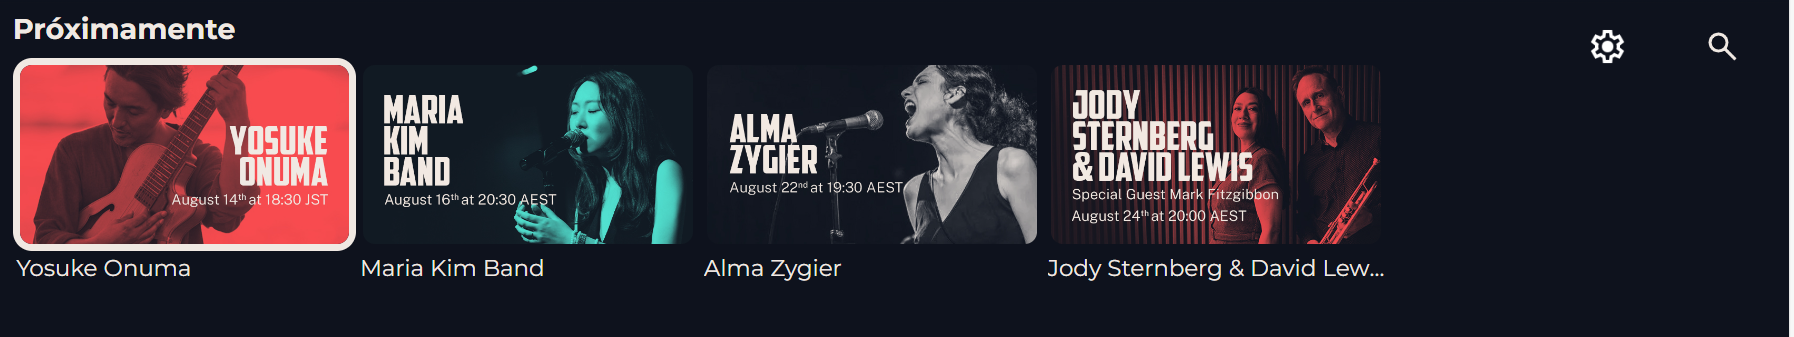
\includegraphics[width=0.8\textwidth]{imaxes/Widget_banner.png}
    \caption{Ejemplo de un widget básico de tipo "banner"}
    \label{fig:Widget_banner}
\end{figure}
\begin{figure}[hp!]
    \begin{subfigure}[c]{0.5\textwidth}
        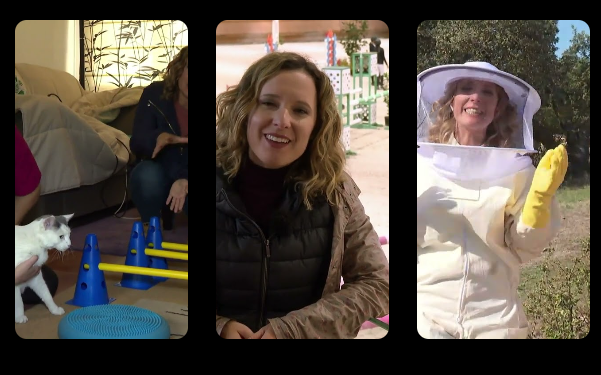
\includegraphics[width=\textwidth]{imaxes/Widget_poster.png}
        \caption{Ejemplo de un widget básico de tipo "poster"}
        \label{fig:Widget_destacado}
    \end{subfigure}
    \hspace{0.1\textwidth}
    \begin{subfigure}[c]{0.5\textwidth}
        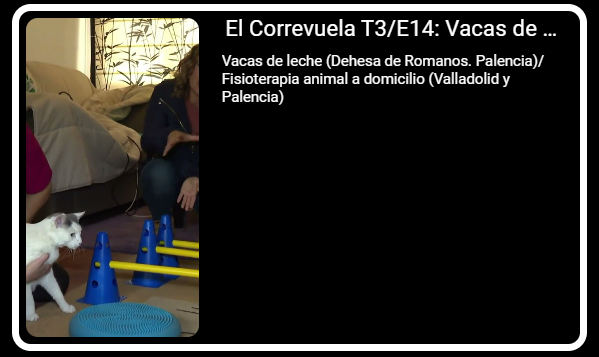
\includegraphics[width=\textwidth]{imaxes/Widget_poster_abierto.png}
        \caption{Ejemplo de un widget básico de tipo "poster" con la información mostrada}
        \label{fig:Widget_poster}
    \end{subfigure}
    \caption{Ejemplos de un widget básico de tipo "poster"}
    \label{fig:Widget_poster}
\end{figure}
\begin{figure}[hp!]
    \centering
    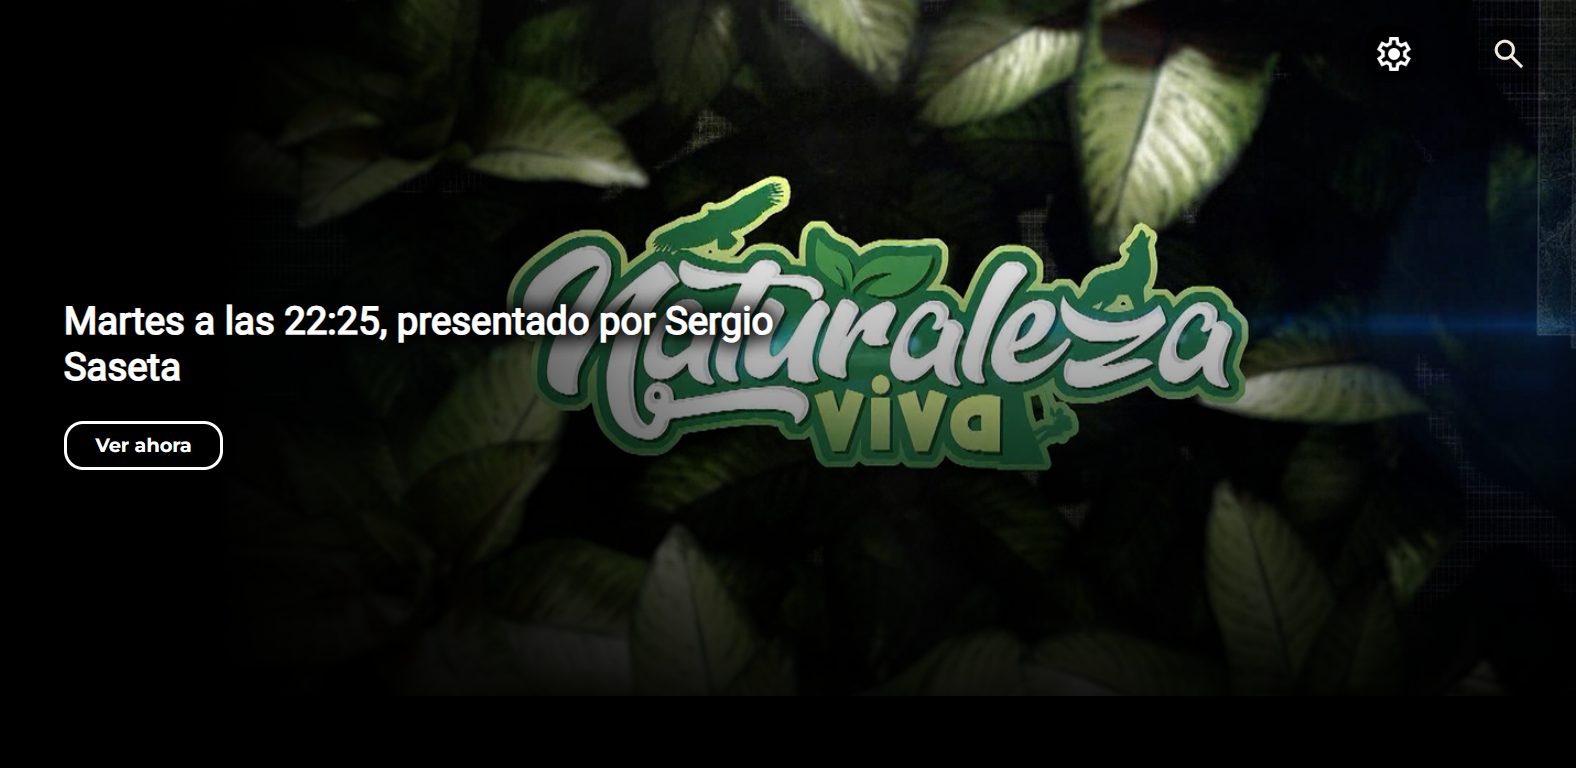
\includegraphics[width=0.8\textwidth]{imaxes/Widget_destacado.png}
    \caption{Ejemplo de un widget básico de tipo "destacado"}
    \label{fig:Widget_mosaico}
\end{figure}

